\documentclass[]{unswthesis}
\usepackage[utf8]{inputenc}
\usepackage{longtable}
\usepackage{array}
\usepackage{multirow}
\usepackage{graphicx}
\usepackage{biblatex}
\addbibresource{pubs.bib}
\usepackage{hyperref}
\usepackage[nottoc]{tocbibind}


%% Thesis details
\thesistitle{Investigating the Effectiveness of Deep Learning Techniques in Forecasting Targeted Mass Killings} 
\thesisschool{School of Computer Science and Engineering}
\thesisschool{School of Computer Science and Faculty of Engineering}
\thesisauthor{Nicolas Blackburn}
\thesisZid{z5163476}
\thesisdegree{Bachelor of Engineering in Software Engineering}

\thesisdate{28 April 2021}
\thesissupervisor{Arcot Sowmya}

%% My own LaTeX macros, definitions, etc
%%%% Shortcuts
\newcommand{\num}[2]{\mbox{#1\,#2}}			% num with units

%%%% Symbols
\newcommand{\yes}{\ensuremath{\surd}\xspace}		% Tick mark
\newcommand{\no}{\ensuremath{\times}\xspace}		% Cross mark
\newcommand{\by}{\ensuremath{\times}\xspace}		% XXX x XXX
\newcommand{\bAND}{\ensuremath{\wedge}\xspace}		% Bool. /\
\newcommand{\bOR}{\ensuremath{\vee}\xspace}		% Bool. \/
\newcommand{\becomes}{\ensuremath{\rightarrow}\xspace}	% -->

%%%% Custom environments

% Centered tabular with single spacing
\newenvironment{ctabular}[1]
    {\par\begin{sspacing}\begin{center}\begin{tabular}{#1}}%
    {\end{tabular}\end{center}\end{sspacing}}


%%%% Our default level for display in TOC - subsubsections
\setcounter{tocdepth}{2}

\documentclass{article}
\usepackage[utf8]{inputenc}
\usepackage[english]{babel}

\usepackage{biblatex}
\addbibresource{pubs.bib}


\begin{document}

%% pages in the ``frontmatter'' section have roman numeral page number
\frontmatter  
\maketitle

\chapter*{Abstract}\label{abstract}


The Target Mass Killing (TMK) dataset is a resource for the study of genocide and other mass atrocities. This project seeks to apply deep learning techniques on the TMK dataset to study and forecast occurrences of TMKs. The project will be build upon pre-existing research that has been done in relation to TMK forecasting. The TMK dataset presents several challenges for traditional deep learning techniques. These challenges include the high levels of class imbalance and high proportion of missing values in the dataset. This project seeks to resolve these issues by data preprocessing techniques and applying a Long Short-Term Memory model to predict occurrences of TMKs.

% \chapter*{Acknowledgements}\label{ack}

This work has been inspired by the labours of numerous academics in
the Faculty of Engineering at UNSW who have endeavoured, over the years, to
encourage students to present beautiful concepts using beautiful
typography.

Further inspiration has come from Donald Knuth who designed \TeX, for
typesetting technical (and non-technical) material with elegance and
clarity; and from Leslie Lamport who contributed \LaTeX, which makes
\TeX\ usable by mortal engineers.

John Zaitseff, an honours student in CSE at the time, created the
first version of the UNSW Thesis \LaTeX\ class and the author of the
current version is indebted to his work.

\chapter*{Abbreviations}\label{abbr}
\begin{description}
\item[BE] Bachelor of Engineering
\item[\LaTeX] A document preparation computer program
\item[PhD] Doctor of Philosophy
\item[AUC] Area Under the Curve
\item[FN] False Negative
\item[FP] False Positive
\item{LSTM} Long Short-Term Memory
\item[PRC] Precision Recall Curve
\item[PITF] Political Instability Task Force 
\item[ROSE] Random Over Sampling Examples
\item[RFE] Recursive Feature Elimination
\item[RNN] Recurrent Neutral Network
\item[SCAD] Social Conflict Analysis Database
\item[SMOTE] Synthetic Minority Oversampling Technique
\item[TN] True Negative
\item[TMK] Targeted Mass Killing
\item[UCDP] Uppsala Conflict Data Program 
\end{description}


\tableofcontents
% \listoffigures  % if required
% \listoftables  % if required

%% pages in the ``mainmatter'' section have arabic page numbers and chapters are numbered
\mainmatter

\chapter{Introduction}\label{ch:intro}

\section{Problem Statement}
"History doesn't repeat itself, but it often rhymes" - Mark Twain

The history of human civilization is soaked in blood and violence. Since the dawn of time, mankind has spent much of our existence waging wars and committing terrible acts of violence against each other. Two thousand years ago the Romans sacked their biter rivals Carthage, butchering half its inhabitants and selling the rest into slavery \cite{carthgeae}. The ancient city was razed to the ground, ensuring Roman hegemony in the Mediterranean. Since then our species evolved and so did our capacity for violence.

The industrial revolution brought on technological advancements that facilitated the execution of mass killings that have never been see before. The Nazi's systematic extermination of the Jewish populations in occupied Europe serves as a truly horrific reminder of what is possible when the resources of a highly industrialized state are coupled with a racist ideology \cite{holocuast}. Even with the end of the World War II and the total defeat of the axis powers ushering a period of increased peace and global stability, there have been numerous recurring episodes of targeted violence across the globe \cite{genocideoccur}. From the valleys of the Balkans during the Yugoslav wars to infamous killing fields of Darfur on the fringes of the Sahara during the Sudanese civil war, these episodes of violence serve as a reminders that targeted mass killings (TMKs) are not a thing of the past. 

Targeted Mass Killings are not spontaneous \cite{JasonBea}. In the lead up to these atrocities a consistent sequence of events usually occurs. This set of reoccurring patterns usually involves the systematic deterioration of socioeconomic factors that ultimately culminate in a TMK episode \cite{Harff2003}. This project seeks to forecast occurrences of TMKs by identifying the patterns of various factors in the lead up to past TMK events.


%The identification and forecasting of mass killings has come a long since Raphael Lemkin first campaigned for genocide to be codified as a international crime in the still nascent United Nations Assembly in 1948. Since then the the study of these mass killings has evolved from a tiny group of scholars to becoming an important function of the United Nations to actively prevent the occurrence of and trail those found responsible.


\section{Aim}
This project aims to assess the effectiveness of applying deep learning methods in predicting Targeted Mass Killings (TMKs)\\

\section{Hypothesis}
\begin{enumerate}
  \item Deep learning methods will be more effective than traditional linear regression techniques in predicting occurrences of TMKs. 
  \item Enriching the existing TMK dataset with additional events will improve TMK forecasting.
\end{enumerate}

\section{Motivation}
Today there are numerous social conflict databases \cite{database} that record and track episodes of tumultuous social upheaval throughout history. Additionally, there have been great improvements in deep learning prediction models. With increased data tracking and advancements in forecasting models, the prediction of TMKs is perhaps more achievable today than at any other point in human history. In recent years some work has been done to attempt to forecast occurrences of genocides that are a subset of TMKs, this work has mostly been driven by political scientists, meaning that there is scope to explore how deep learning can improve current forecasting models. This project hopes to extend on the work of Goldsmith and Butcher (2018): \emph{Genocide Forecasting Accuracy and New Forecasting to 2020} \cite{Goldsmith2018} where linear regression models were applied.

An objective of this project is to utilize deep learning techniques to predict episodes of TMKs. Up to this point the application of deep learning in social sciences is relatively rare and it is hoped that they will be a useful tool in forecasting such killings.


\chapter{Literature Review}\label{ch:background}

\section{Targeted Mass Killings (TMKs)}
\subsection{Definitions}
This project will use the TMK definition provided by Goldsmith, Butcher, Nanlohy and Muchlinski in their paper \emph{Targeted Mass Killing dataset}. A TMK is defined as \emph{“is the direct killing of non-combatant members of a
group by a formally organized armed force that results in 25 or more deaths in an annual period,
with the intent of destroying the group or intimidating the group by creating a perception of
imminent threat to its survival. A targeted group is defined in terms of political and/or ethnic and/or
religious identity.”}

\section{Previous work}
Several key factors have been identified as 


\section{Deep Learning}|
\subsection{Defin}

\section{Class Imbalance}
\subsection{Definition}
The classification of imbalanced data
In our case the minority instances of TMKs actua
Most deep learning techniques perform poorly in classifying datasets if class-to-clashttps://www.overleaf.com/project/6077bd90e4c2db93be17f470s separability is poor due to strong bias towards the majority class.


\subsection{Imbalance Ratio}
The Imbalance ratio is used to quantity the maximum between-class imbalance level. $C_i$ is a set of example in class $i$. $max_i{|C_i|}$ and $min_i{|C_i|}$ represent the maximum and minimum number of instances from class \emp{i} respectively. In a binary classification problem where the majority class has 500 instances and the minority has 100, the imbalance ratio $\rho = 5$\\

$\rho = \frac{max_i\{|C_i|\}}{min_i\{|C_i|\}}$

\subsection{Consequences of High Class Imbalance}
\chapter{Data}\label{ch:style}
\section{TMK Dataset}

The TMK dataset was created by Goldsmith, Butcher, Benjamin, Sowmya, Muchlinski (2020) in  \emph{“Introducing The Targeted Mass Killing Dataset for the Study and Forecasting of Mass Atrocities”} \cite{Goldsmith2013}
The TMK dataset was created to contribute to the study into various atrocities such as genocide and politicide. 

The TMK dataset records events from 1946-2019 and tracks a wide variety of socioeconomic factors. The scale of the TMK event is quantified via a pre-coded ordinal indicator that aggregates evidence of intent as well as number of deaths. The scale and corresponding criteria for that classification is shown in Table 3.1. If time permits this project will try to produce a model that attempts to predict the severity of the TMK via the TMK ordinal indicator.
\begin{center}
\begin{table}
\begin{center}
 \begin{tabular}{||c c c||} 
 \hline
 Score & Intent & Total Deaths\\ [1ex] 
 \hline
 1 & NO Stated OR Organizational Intent & $25 \leq x \leq 999$ \\ [1ex] 
 \hline
 2 & NO Stated OR Organizational Intent &  $\geq 1000$  \\ [1ex] 
 \hline
 3 & Stated OR Organizational Intent & $25 \leq x \leq 999$ \\ [1ex]  
 \hline
  & TMK GENOCIDE/POLITICIDE THRESHOLD & \\
 \hline
 4 & Stated AND Organizational Intent  &  $\geq 1000$  \\ [1ex] 
 \hline
  5 & Stated AND Organizational Intent  & $25 \leq x \leq 999$  \\ [1ex] 
 \hline
  6 & Stated AND Organizational Intent  &  $\geq 1000$   \\ [1ex] 
 \hline
  7 & Stated AND Organizational Intent  &  $\geq 10,000$   \\ [1ex] 
 \hline
  8 & Stated AND Organizational Intent  &  $\geq 100,000$   \\ [1ex] 
 \hline
\end{tabular}
\caption{TMK Severity}
\end{center}
\end{table}
\end{center}
\pagebreak
\subsection{Generating Training Dataset}
The training dataset for my model will be generated using the following steps
\begin{enumerate}
  \item Merge selected variables from TMK events with some other datasets.
  \item Remove duplicated rows.
  \item Created lagged target variables because It takes time for some factors to take effect.
\end{enumerate}

The process of generating training datasets this way has been done before by others and produced a dataset with an imbalanced ratio $\rho = 26$ which translates to about 96\% non-tmk events. An imbalanced ratio of this magnitude is to be expected in this project's training dataset.

\section{Alternative Data Sources}
\subsection{Social Conflict Analysis Database}
The Social Conflicts Analysis Database(SCAD) includes protests, riots, strikes, inter-communal conflicts, government violence against civilians and other forms of social conflict not systematically tracked in other conflict datasets. SCAD currently includes information social conflicts from 1990-2017, covering all of Africa and now also Mexico, Central America, and the Caribbean.
\subsection{Uppsala Conflict Data Program}
The Uppsala Conflict Data Program (UCDP) is the world’s main provider of data on organized violence and the oldest ongoing data collection project for civil war, with a history of almost 40 years. Its definition of armed conflict has become the global standard of how conflicts are systematically defined and studied.
\subsection{Political Instability Task Force}
The Political Instability Task Force (PITF) is a U.S government project to construct a database on major domestic political conflicts leading up to state failures. Some variables that are tracked include the strength of a nations institutions and various social economic indicators such as infant mortality and life expectancy.
web-pages~\cite{Noo05}.
only.


\begin{figure}[h]
\centering
\includegraphics{data_compare.png}
\caption{Data Sources Comparison}
\end{figure}

A preliminary investigation of each other data sources has been conducted and it has been concluded that the SCAD database will be used in conjunction with the TMK dataset. This is mostly due to the high number of overlapping variables between the datasets. This makes merging the two via a full outer join easier as there will be less variables in the resultant dataset
\section{Data Issues}
\subsection{Class Imbalance}
As established in the literature review occurrences of TMKs are very rare and the generated training dataset is expected to have an imbalance ratio $\rho \approx  26$. There are a number of techniques that will be applied to resolve the class imbalance problem.

\subsubsection{Upsampling}
A common way of resolving the problem of class imbalance is upsampling where synthetic datapoints are artificially generated from the minority class

\begin{figure}[h]
\centering
\includegraphics{oversampling.png}
\caption{Upsampling}
\end{figure}

\subsubsection{Random Over-Sampling Examples(ROSE)}

The ROSE R package implements simple upsampling which involves populating empty features with zero-valued samples. ROSE also provides more robust upsampling where new datapoints are generated from the minority class based on the probability distribution and co-variance of the dataset. ROSE produces a \emph{"considerable amount of repeated observations amongst the rare examples"} ” (Lunardon, Menardi and Torelli, 2015, p84) \cite{Lunardo}. The ROSE algorithm is outlined in the figure below

\begin{figure}[h]
\centering
\includegraphics{rose_algo.png}
\caption{ROSE Algorithm}
\end{figure}

A weakness of ROSE is that if a large number of new data points are generated from a small subset of points it can lead to over fitting which will cause an increased generalization error (Fernandez et al, 2018, p83) \cite{Fernandez}. 

\subsubsection{Synthetic Minority Oversampling Technique(SMOTE)} 

\begin{figure}[h]
\centering
\includegraphics{knn.png}
\caption{SMOTE knn}
\end{figure}

Another technique for the generation of synthetic datapoints from the minority class is SMOTE. SMOTE randomly selects an instance from the minority class and applies the k nearest neighbours \cite{smotefamily}. A new datapoint is created by randomly selecting one the k nearest neighbours and connecting the two data points in the feature space. The new instance is generated as a convex combination of the two chosen instances. This allows new datapoints to be created based on topological properties in the neighborhood of the minority class, resulting in realistic datapoints. Figure 3.4 depicts how new datapoints are created in between the k nearest neighbours of the selected point.

\subsubsection{Downsampling}
An alternative to resolving the class imbalance problem without using upsampling is downsampling. Downsampling selects a subset of the majority class, this subset will be the same size as the minority class to ensure no class dominates the other. The selection of the subset is performed randomly.

\begin{figure}[h]
\centering
\includegraphics{downsampling.png}
\caption{Downsampling}
\end{figure}

The advantages of the downsampling is that it is very simple to perform and downsampling techniques are easily accessible via the R library ROSE. Additionally no overfitting will occur which is the case for upsampling techniques.

Disadvantages of downsampling are that potentially important information is lost from the datapoints of the majority class that are discarded, resulting in the model not being able to train on some features. Additionally if the class imbalance is very high there will only be a small pool of minority samples that are of greater interest to the model. Since the number of majority samples must be the same size as the ones from the minority class, the resultant dataset will be tiny and will not contain enough data for the model to train on


\subsubsection{Strategy for Resolving Class Imbalance}
This project will apply both ROSE, SMOTE and downsampling to resolve the class imbalance issue. As the literature states that a combination of techniques produces the most robust dataset.\emph{"The combination of SMOTE and under-sampling performs better than plain under-sampling"} \cite{Lunardo}.By using a combination of techniques the downsides of individual techniques such as over-fitting and lost of important information will be mitigated.

\subsection{Missing Values}
Like most datasets in social science a lot of TMK events have missing values across various features. Fig 3.6 depicts a sample of some of the features in the TMK dataset and the percentage of missing values across all the events. 

\begin{figure}[h]
\centering
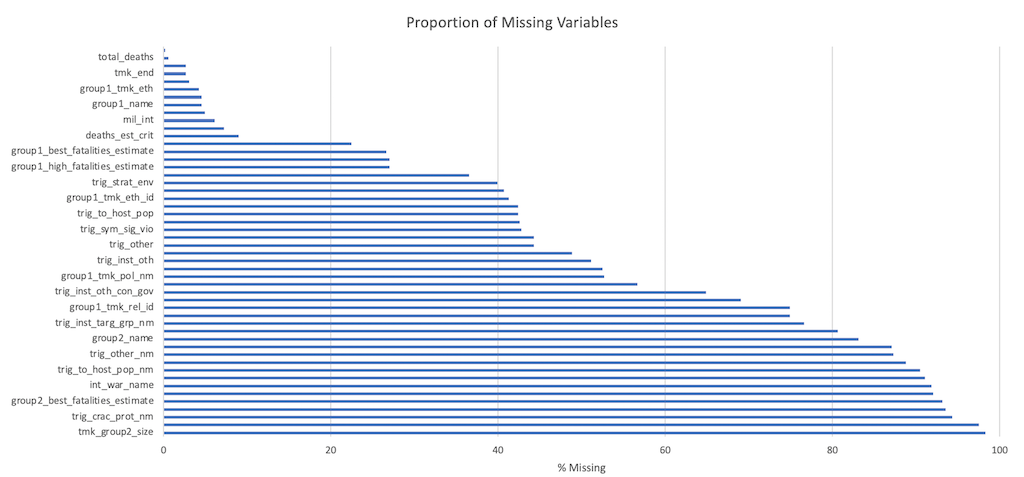
\includegraphics{proportionOfMissingvalues.png}
\caption{Proportion of missing values in TMK dataset}
\end{figure}


\subsubsection{Logical Imputations}
Logical imputation involves replacing missing values when the logic is obvious. For example, missing values can be logically imputated for TMK related because the dataset contains only TMK events.

\subsubsection{Multivariate Imputation Chained Equations}
Multivariate Imputation via Chained Equations (MICE) comprises of two techniques as outlined by Van Buren (2018) \cite{vanBuren}. The database contains missing values that match a \emph{"general pattern of missing data"}. 

MICE implements two methods for imputation of missing values. The first is Joint Modelling(JM) where imputations are drawn from a multivariate model fitted to data. The second is Fully Conditional Specification (FCS) involves drawing imputations from iterated conditional models. 

Both JM and FCS are available in R via the MICE package. A limitation of using the MICE package is that it can affect the bias and standard error of the data.

\begin{figure}[h]
\centering
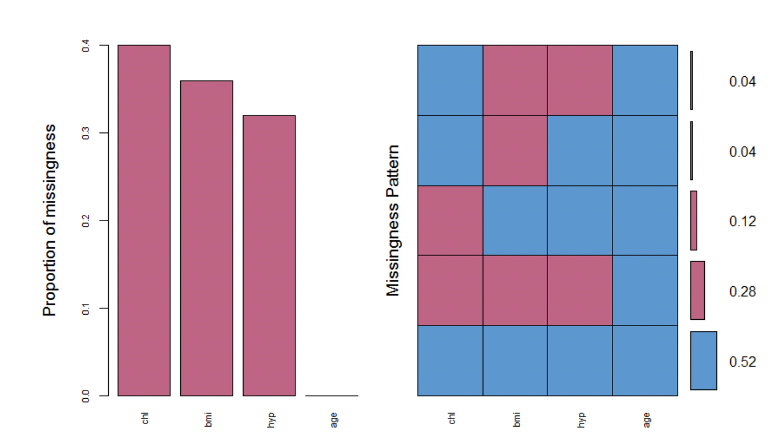
\includegraphics{missingdataimage.png}
\caption{General pattern of missing data visualized. Missing data in red}
\end{figure}


\subsection{Feature Explosion}
The TMK dataset already contains 121 different features. When additional datasets are merged via an outer join the number of features will only increase. When a model has to train on too many features it will encounter difficulty in identifying important features from less useful ones. This is known as the curse of dimensionality. 

To deal with the problem of feature explosion we will apply the Recursive Feature Elimination Algorithm(RFE) which is availability in the sklearn framework in python. 

As depicted in Fig 3.8 the RFE  algorithm recursively removes features at each step and re-ranks remaining features by retraining support vector machines based on these remaining features. If a feature is a weak feature, RFE will simply remove it. This apporach may present issues, because a weak feature may still be an important feature when used in conjunction with other features. 

\begin{figure}[h]
\centering
\includegraphics{rfe.png}
\caption{Recursive Feature Elimination Algorithm \cite{Furianello}}
\end{figure}

\chapter{Methods}\label{ch:eval}


\section{Programming Languages}

\subsection{R}
R will be use for primarily for the preprocessing of data, this encompasses the ge

% \begin{center}
% \begin{tabular}{ |c|c } 
% \hline
% R library & Description \\
% \hline
% \multirow{3}{4em}{smotefamily} & \multirow{3}{4em}{Multiple row SMOTE is a oversampling technique which synthesizes a new minority instance  between a pair of one minority instance and one of its K nearest neighbor} \\ 
% rose & cell8 \\ 
% mice & cell8 \\ 
% \hline
% \end{tabular}
% \end{center}


 \begin{longtable}[c]{| c | l |}
 \caption{Long table caption.\label{long}}\\

 
 \hline
 R library & Description\\
 \hline
 \endfirsthead

 \hline
 \multicolumn{2}{|l|}{Continuation of Table \ref{long}}\\
 \hline
 R library & Descriptiom\\
 \hline
 \endhead

 \hline
 \endlastfoot

smotefamily & SMOTE is a oversampling technique which synthesizes a new minority instance  \\
& between a pair of one minority instance and one of its K nearest neighbors\\
 \hline
rose & The package provides functions to deal with binary classification problems in the \\
& presence of imbalanced classes. Synthetic balanced samples are generated \\ 
& according to ROSE (Menardi and Torelli, 2013).\\
 \hline
 mice & Multiple imputation using Fully Conditional Specification (FCS) implemented \\
 & by the MICE algorithm as described in Van Buuren and Groothuis \\ 
 & Oudshoorn(2011)
 \end{longtable}


\section{Discussion}

\chapter{Project Plan}\label{ch:projectplan}
\section{Thesis A Progress}
Apart from conducting a literature review for the thesis, an investigation was undertaken to determine the best social conflict databases that would be the best for merging with the TMK dataset. Additionally a Linux machine has been set up on CSE and has been populated with a test dataset. A simple multi-layer perception model has also been created and run on the test data. The model was trained on unprocessed data so naturally the model performed poorly, its purpose was more to test if neural networks could be run on the dataset with all its variables in a reasonable amount of time.
\subsection{Deliverables}
The deliverables for thesis A are the seminar in (week 8) and the report (week 10)
\section{Thesis B Plan}
\subsection{Generate Dataset(2 weeks)}
The dataset will be generated via merging the TMK events with external datasets as outlined in the 
\subsection{Data processing(2 weeks)}
Synthetic data will be generated to account for the level of class imbalance in the dataset. Synthetic data-points will be created via the R libraries of ROSE and SMOTE. Downsmapling will also be conducted to reduce the level of class imbalance as well as mitigate the level of over-fitting via ROSE and SMOTE. Finally once the issue of class imbalance has been resolved the imputation of missing values in the dataset will be completed via the MICE package in R.

\subsection{Creating the Model(5 weeks)}
The keras framework in python will be used to code to LSTM model

\subsection{Backup Plan}
If the LSTM model performs poorly alternative architectures will be used. 
\begin{itemize}
  \item Convolutional Neural Network (CNN)
  \item Vector Auto Regression (VAR)
  \item Auto-encoder
\end{itemize}
\subsubsection{Backup Plan}
If there are  significant issues with all the of the listed models, the forecasting of TMKs via deep learning will be abandoned and a Random Forest model will be used.

\section{Thesis C Plan}
Research ideas for thesis C are dependant on the performance of models created in thesis B
\subsection{Output Risks}
The output of LSTM model created in thesis B can be modified to output a calculated risk of a TMK occurring instead of a binary prediction. The plan is for the model to output a percentage likelihood from 0-100\% of a TMK occurring in a particular country for a selected year.

\subsection{Predict Severity}
The TMK dataset has a ordinal indicator that quantifies the severity of a TMK event. The ordinal indicator is a value from 1 to 8 with 1 being an event that just meets the minimum requirements of a TMK event and 8 being a high-severity event with over 100,000 deaths and the perpetrators were a state who conducted the TMK with organizational intent.

\subsection{Investigate Other Models}
Depending on the difficulty as well as time constraints, it would be useful to see how different deep learning models perform against each other in the newly generated dataset. Some alternative neural networks that would be interesting to compare against the LSTM include the Convolutional Neural Network, Multi-Layer Perception (MLP) and generic Recurrent Neural Network (RNN). Additionally the architectures of Vector Auto Regression (VAR) and Auto-encoders would be interesting.

\subsection{Fine Tune Model}
The aim of the thesis is to obtain the best deep learning model for forecasting occurrences of TMK events. Naturally a significant proportion of time will be used to experiment and adjust hyper-parameters to produce the best model. Some hyper-parameters that will be adjusted accordingly include learning rate, dropout, stride, activation function and many others.





%% chapters in the ``backmatter'' section do not have chapter numbering
%% text in the ``backmatter'' is single spaced
\backmatter
% \bibliographystyle{alpha}
% \bibliography{pubs}
\printbibliography


\end{document}
